%%%%%%%%%%%%%%%%%%%%%%%%%%%%%%%%%%%%%%%%%%%%%%%%%%%%%%%%%%%%%%%%%%%%%
%% This is a (brief) model paper using the achemso class
%% The document class accepts keyval options, which should include
%% the target journal and optionally the manuscript type. 
%%%%%%%%%%%%%%%%%%%%%%%%%%%%%%%%%%%%%%%%%%%%%%%%%%%%%%%%%%%%%%%%%%%%%
\documentclass[journal=jacsat,manuscript=article]{achemso}
%\documentclass[12pt]{article}
%\usepackage[letterpaper,left=0.5in,right=0.5in,top=1.0in,bottom=1.0in]{geometry}

%%%%%%%%%%%%%%%%%%%%%%%%%%%%%%%%%%%%%%%%%%%%%%%%%%%%%%%%%%%%%%%%%%%%%
%% Place any additional packages needed here.  Only include packages
%% which are essential, to avoid problems later. Do NOT use any
%% packages which require e-TeX (for example etoolbox): the e-TeX
%% extensions are not currently available on the ACS conversion
%% servers.
%%%%%%%%%%%%%%%%%%%%%%%%%%%%%%%%%%%%%%%%%%%%%%%%%%%%%%%%%%%%%%%%%%%%%
\usepackage[version=3]{mhchem} % Formula subscripts using \ce{}
\usepackage{siunitx} % generating degrees Celsius in the document 
\usepackage{color}
\usepackage{soul} % allows highlighting text 
\usepackage{makecell}
\usepackage{booktabs}
\usepackage{amsmath}
\usepackage{amssymb}
\usepackage{todonotes}
\usepackage{gensymb}
\usepackage{verbatim}
\usepackage{hyperref}
\hypersetup{
    colorlinks=true,
    citecolor= red,
    linkcolor=blue,
    urlcolor=blue, 
    breaklinks=true
}

%%%%%%%%%%%%%%%%%%%%%%%%%%%%%%%%%%%%%%%%%%%%%%%%%%%%%%%%%%%%%%%%%%%%%
%% If issues arise when submitting your manuscript, you may want to
%% un-comment the next line.  This provides information on the
%% version of every file you have used.
%%%%%%%%%%%%%%%%%%%%%%%%%%%%%%%%%%%%%%%%%%%%%%%%%%%%%%%%%%%%%%%%%%%%%
%%\listfiles

%%%%%%%%%%%%%%%%%%%%%%%%%%%%%%%%%%%%%%%%%%%%%%%%%%%%%%%%%%%%%%%%%%%%%
%% Place any additional macros here.  Please use \newcommand* where
%% possible, and avoid layout-changing macros (which are not used
%% when typesetting).
%%%%%%%%%%%%%%%%%%%%%%%%%%%%%%%%%%%%%%%%%%%%%%%%%%%%%%%%%%%%%%%%%%%%%
\newcommand*\mycommand[1]{\texttt{\emph{#1}}}
\DeclareRobustCommand
  \Compactcdots{\mathinner{\cdotp\mkern-2mu\cdotp\mkern-2mu\cdotp}}

%%%%%%%%%%%%%%%%%%%%%%%%%%%%%%%%%%%%%%%%%%%%%%%%%%%%%%%%%%%%%%%%%%%%%
%% Meta-data block
%% ---------------
%% Each author should be given as a separate \author command.
%%
%% Corresponding authors should have an e-mail given after the author
%% name as an \email command. Phone and fax numbers can be given
%% using \phone and \fax, respectively; this information is optional.
%%
%% The affiliation of authors is given after the authors; each
%% \affiliation command applies to all preceding authors not already
%% assigned an affiliation.
%%
%% The affiliation takes an option argument for the short name.  This
%% will typically be something like "University of Somewhere".
%%
%% The \altaffiliation macro should be used for new address, etc.
%% On the other hand, \alsoaffiliation is used on a per author basis
%% when authors are associated with multiple institutions.
%%%%%%%%%%%%%%%%%%%%%%%%%%%%%%%%%%%%%%%%%%%%%%%%%%%%%%%%%%%%%%%%%%%%%
\author{Stephen P. Vicchio}
\affiliation[Clemson University]
{Department of Chemical and Biomolecular Engineering, Clemson University, Clemson, SC}
\author{Zhihengyu Chen}
\affiliation[Stony Brook University]
{Department of Chemistry, Stony Brook University, Stony Brook, NY}
\author{Karena Chapman}
\email{karena.chapman@stonybrook.edu}
\affiliation[Stony Brook University]
{Department of Chemistry, Stony Brook University, Stony Brook, NY}
\author{Rachel B. Getman}
\email{rgetman@g.clemson.edu}
\affiliation[Clemson University]
{Department of Chemical and Biomolecular Engineering, Clemson University, Clemson, SC}

%%%%%%%%%%%%%%%%%%%%%%%%%%%%%%%%%%%%%%%%%%%%%%%%%%%%%%%%%%%%%%%%%%%%%
%% The document title should be given as usual. Some journals require
%% a running title from the author: this should be supplied as an
%% optional argument to \title.
%%%%%%%%%%%%%%%%%%%%%%%%%%%%%%%%%%%%%%%%%%%%%%%%%%%%%%%%%%%%%%%%%%%%%
\title[manuscript]{
Identifying the structure and composition of \ce{Ni(II)}-hydroxo catalyst supported the NU-1000 metal-organic framework
}

%%%%%%%%%%%%%%%%%%%%%%%%%%%%%%%%%%%%%%%%%%%%%%%%%%%%%%%%%%%%%%%%%%%%%
%% Some journals require a list of abbreviations or keywords to be
%% supplied. These should be set up here, and will be printed after
%% the title and author information, if needed.
%%%%%%%%%%%%%%%%%%%%%%%%%%%%%%%%%%%%%%%%%%%%%%%%%%%%%%%%%%%%%%%%%%%%%
\abbreviations{IR,NMR,UV}
\keywords{American Chemical Society, \LaTeX}

%%%%%%%%%%%%%%%%%%%%%%%%%%%%%%%%%%%%%%%%%%%%%%%%%%%%%%%%%%%%%%%%%%%%%
%% The manuscript does not need to include \maketitle, which is
%% executed automatically.
%%%%%%%%%%%%%%%%%%%%%%%%%%%%%%%%%%%%%%%%%%%%%%%%%%%%%%%%%%%%%%%%%%%%%
\begin{document}

%%%%%%%%%%%%%%%%%%%%%%%%%%%%%%%%%%%%%%%%%%%%%%%%%%%%%%%%%%%%%%%%%%%%%
%% The "tocentry" environment can be used to create an entry for the
%% graphical table of contents. It is given here as some journals
%% require that it is printed as part of the abstract page. It will
%% be automatically moved as appropriate.
%%%%%%%%%%%%%%%%%%%%%%%%%%%%%%%%%%%%%%%%%%%%%%%%%%%%%%%%%%%%%%%%%%%%%
%\begin{tocentry}
%
%Some journals require a graphical entry for the Table of Contents.
%This should be laid out ``print ready'' so that the sizing of the
%text is correct.
%
%Inside the \texttt{tocentry} environment, the font used is %Helvetica
%8\,pt, as required by \emph{Journal of the American Chemical
%Society}.
%
%The surrounding frame is 9\,cm by 3.5\,cm, which is the maximum
%permitted for  \emph{Journal of the American Chemical Society}
%graphical table of content entries. The box will not resize if the
%content is too big: instead it will overflow the edge of the box.
%
%This box and the associated title will always be printed on a
%separate page at the end of the document.
%
%\end{tocentry}

%%%%%%%%%%%%%%%%%%%%%%%%%%%%%%%%%%%%%%%%%%%%%%%%%%%%%%%%%%%%%%%%%%%%%
%% The abstract environment will automatically gobble the contents
%% if an abstract is not used by the target journal.
%%%%%%%%%%%%%%%%%%%%%%%%%%%%%%%%%%%%%%%%%%%%%%%%%%%%%%%%%%%%%%%%%%%%%
\begin{abstract}
Metal-organic frameworks (MOFs) provide an excellent platform for supporting 3d transition metal complexes. Despite being catalytically active for gas-to-liquid transformations of natural gas, open questions about the exact structure of the catalytically-active state of the metal complex inhibit our ability to rationally design these catalysts. These supported metal cation complexes exhibit structures changes that affect catalytic performance when exposed to different reaction environments (such as an increase in temperature and exposure to \ce{H2} gas). Therefore, to reach their full-potential as catalytic materials, fundamental insights into the relationship between reaction environment, structure, and performance are required. We use a combined density functional theory (DFT) and \textit{ab initio} thermodynamic analysis to determine the structure and composition of a tetranuclear \ce{Ni} metal complex supported on NU-1000. Here we show that the lowest energy structural and compositional arrangement of the \ce{Ni} cluster is highly sensitive to reaction conditions (temperature, \ce{H2O} partial pressure, and \ce{H2} partial pressure) using phase diagrams, which reveal the thermodynamic landscape of the \ce{Ni} cluster. We compare the local atomic structures of our thermodynamic models to experimentally local structural information obtained by differential pair distribution functions (dPDFs). By comparing the local structural information for model structures and experimental data, specifically the \ce{Ni-O}, \ce{Ni{\Compactcdots}Ni}, and \ce{Ni{\Compactcdots}Zr} atomic distances, we demonstrate the importance of \ce{H2O} within the \ce{Ni} metal complex active site in maintaining a high \ce{Ni} coordination. We find highly coordinated structures show much better agreement to the experimental data. Our computational modeling demonstrates how the catalyst structure is controlled by temperature and partial pressure. The findings establish thermodynamically relevant models that require further computational catalytic investigations as well as showcasing how to tune structures using different reaction conditions.
\end{abstract}

%%%%%%%%%%%%%%%%%%%%%%%%%%%%%%%%%%%%%%%%%%%%%%%%%%%%%%%%%%%%%%%%%%%%%
%% Start the main part of the manuscript here.
%%%%%%%%%%%%%%%%%%%%%%%%%%%%%%%%%%%%%%%%%%%%%%%%%%%%%%%%%%%%%%%%%%%%%

\section{Introduction}
A challenge within catalysis research is converting light hydrocarbons (mainly methane, ethane, and propane) into longer chain hydrocarbons (\ce{C6} to \ce{C10}) or alcohols. These gas-to-liquid (GTL) chemical transformations require a series of catalytic reactions involving hydrogenation, oligomerization, dimerization, and/or partial oxidation steps to generate the desired products. Industrially, hydrocarbon transformations are often performed using homogeneous catalysts,\cite{Speiser2005, Maji2017} such as the \ce{Ni} complex within the Shell higher oligomers process (SHOP).\cite{Reuben1988} Homogeneous catalyst are attractive for catalysis because they feature isolated metal sites in a well-defined environment created by the ligand coordination and demonstrate high metal utilization. Traditionally, heterogeneous catalytic materials lack the advantages exhibited by homogeneous systems. However, recent scientific advancements are ushering in a new era of heterogeneous catalysts designed to mimic the isolated active sites of homogeneous catalysts while anchored to a solid support.\cite{Kaiser2020}

Chemical reactions on traditional heterogeneous catalysts usually occurs at the surface of a solid catalyst where on a small number of metal atoms actually participate in the reaction. The exact geometric and electronic nature of the active site is often unknown or difficult to elucidate for traditional heterogeneous catalysts. Newly envisioned heterogeneous catalytic materials, called single-atom catalysts (SACs), address these limitations. Broadly, SACs contain atoms of any element that are spatially and electronically isolated from chemically identical atoms and anchored to a solid support.\cite{Kaiser2020,Qiao2011,Cui2017,Yang2013} Atomically dispersing the atoms, often 3d transition metals,\cite{Kaiser2020} to a solid support leads to improved metal utilization and generates a more well-defined active site structures for SACs. SACs aren't restricted to a single-type of solid support; atomically dispersed metal atoms have been generated on metal-organic frameworks (MOFs),\cite{Zheng2019,AbdelMageed2019,Huang2019} bulk metals,\cite{Patel2019,Pei2017,Qian2012} metal oxides,\cite{Bo2019,Jiao2019,Riley2018,Tang2019} zeolites,\cite{Mao2016, Kistler2014} and covalent-organic frameworks (COFs),\cite{Zhong2019,Romero-Muniz2020} The structure of the active site on these various supports is defined by the dispersed metal species, coordinating ligands, and steric environment with these factors contributing to the reactivity and selectivity of the catalyst. Furthermore, an ensemble of active site structures containing varying nuclearity is observed depending on the dispersed metal atoms and support used. The diversity and tunable of SACs offers new catalysts with interesting reactivity and selectivity, but difficulties in determining the precise active structure poise significant limitations in catalyst design. 

The exact structure of the active site for SACs is further complicated by the influence of reaction conditions. For traditional heterogeneous catalyst, the influence of reaction conditions on the catalyst surface properties are well known. The surface coverages of different gas phase species has been extensively investigated on a variety of metal surfaces.\cite{Getman2008,Piccinin2017,Zuo2016,Bray2015} However, in SACs systems the reaction conditions not only impact surface coverages, but also structural changes that define the catalytic mechanism.\cite{Kim2015,Redfern2018,Mian2020,Shabbir2020} Given catalyst structure drives catalyst function, there is a growing need to understand how the reaction environment transforms the active site structure of SACs under a variety of conditions.\cite{Tang2019} The unambiguous determination of SACs active site structure remains an ongoing challenge, with rational catalyst design inhibited by difficulties in determining the precise active site. 

Our work investigates how the reaction environment (temperature and gas phase conditions) influence the structure of SACs supported on the NU-1000 metal-organic framework (MOF). MOFs, a porous crystalline material formed from inorganic nodes interconnected by organic linkers,\cite{Furukawa2013,Li1999} are commonly used to support 3d transition metal complexes as single-atom catalysts.\cite{Cui2018, Noh2016, Li2017, Song2019, Nguyen2015, Hackler2020} Metal complexes, comprised of metal atoms (e.g., \ce{Ni(II)}) and coordinating ligands (e.g., \ce{OH}/\ce{OH2}), generate the active site species. However, elucidating the exact structure of the active site is challenging and further complicated by structural changes induced by the reaction environment.\cite{PlateroPrats2017b,Rimoldi2017} We address these ongoing questions about the exact structure of a \ce{Ni(II)} metal complex supported on NU-1000 when exposed to \ce{H2} gas. Herein we combine density functional theory (DFT) calculations and gas phase empirical models to perform \textit{ab initio} thermodynamic analysis to calculate the stability of a \ce{Ni4}-cluster supported on NU-1000 under different temperatures and gas phase conditions (\ce{H2} and \ce{H2O}). Modeling reveals the thermodynamic landscape of the \ce{Ni4}-cluster under different conditions. We further investigate our model by comparing the local structural information of thermodynamic relevant structures to experimental structures. Our results provide structural information about the types of changes exhibited by the cluster to establish more appropriate molecular models, such as the role of \ce{H2O} within the active site.  

%%%%%%%%%%%%%%%%%%%%%%%%%%%%%%%%%%%%%%%%%%%%%%%%%%%%%%%%%%%%%%%%%%%%%
%% Methodology
%%%%%%%%%%%%%%%%%%%%%%%%%%%%%%%%%%%%%%%%%%%%%%%%%%%%%%%%%%%%%%%%%%%%%
\section{Methodology}
The zirconium based MOF NU-1000 is commonly used as a catalyst support for 3d transition metal complexes.\cite{Shabbir2020, Hackler2020, Ortuno2016, Pellizzeri2018} NU-1000 is comprised of zirconium-oxide nodes connected by carbon-based pyrene linkers. The resulting crystal structure contains large hexagonal channels (31 {\AA}), triangular channels (10 {\AA}), and small pores (8 {\AA}) as shown in Figures~\ref{fig:Ni-MOF-model}a and~\ref{fig:Ni-MOF-model}b. The unit cell is hexagonal with optimized parameters of $a=b=40.611$ {\AA}, $c=15.990$ {\AA}, $\alpha=\beta=\ang{90}$, and $\gamma=\ang{60}$, in agreement with prior work.\cite{PlateroPrats2017} 

\begin{figure}[H]
    \centering
    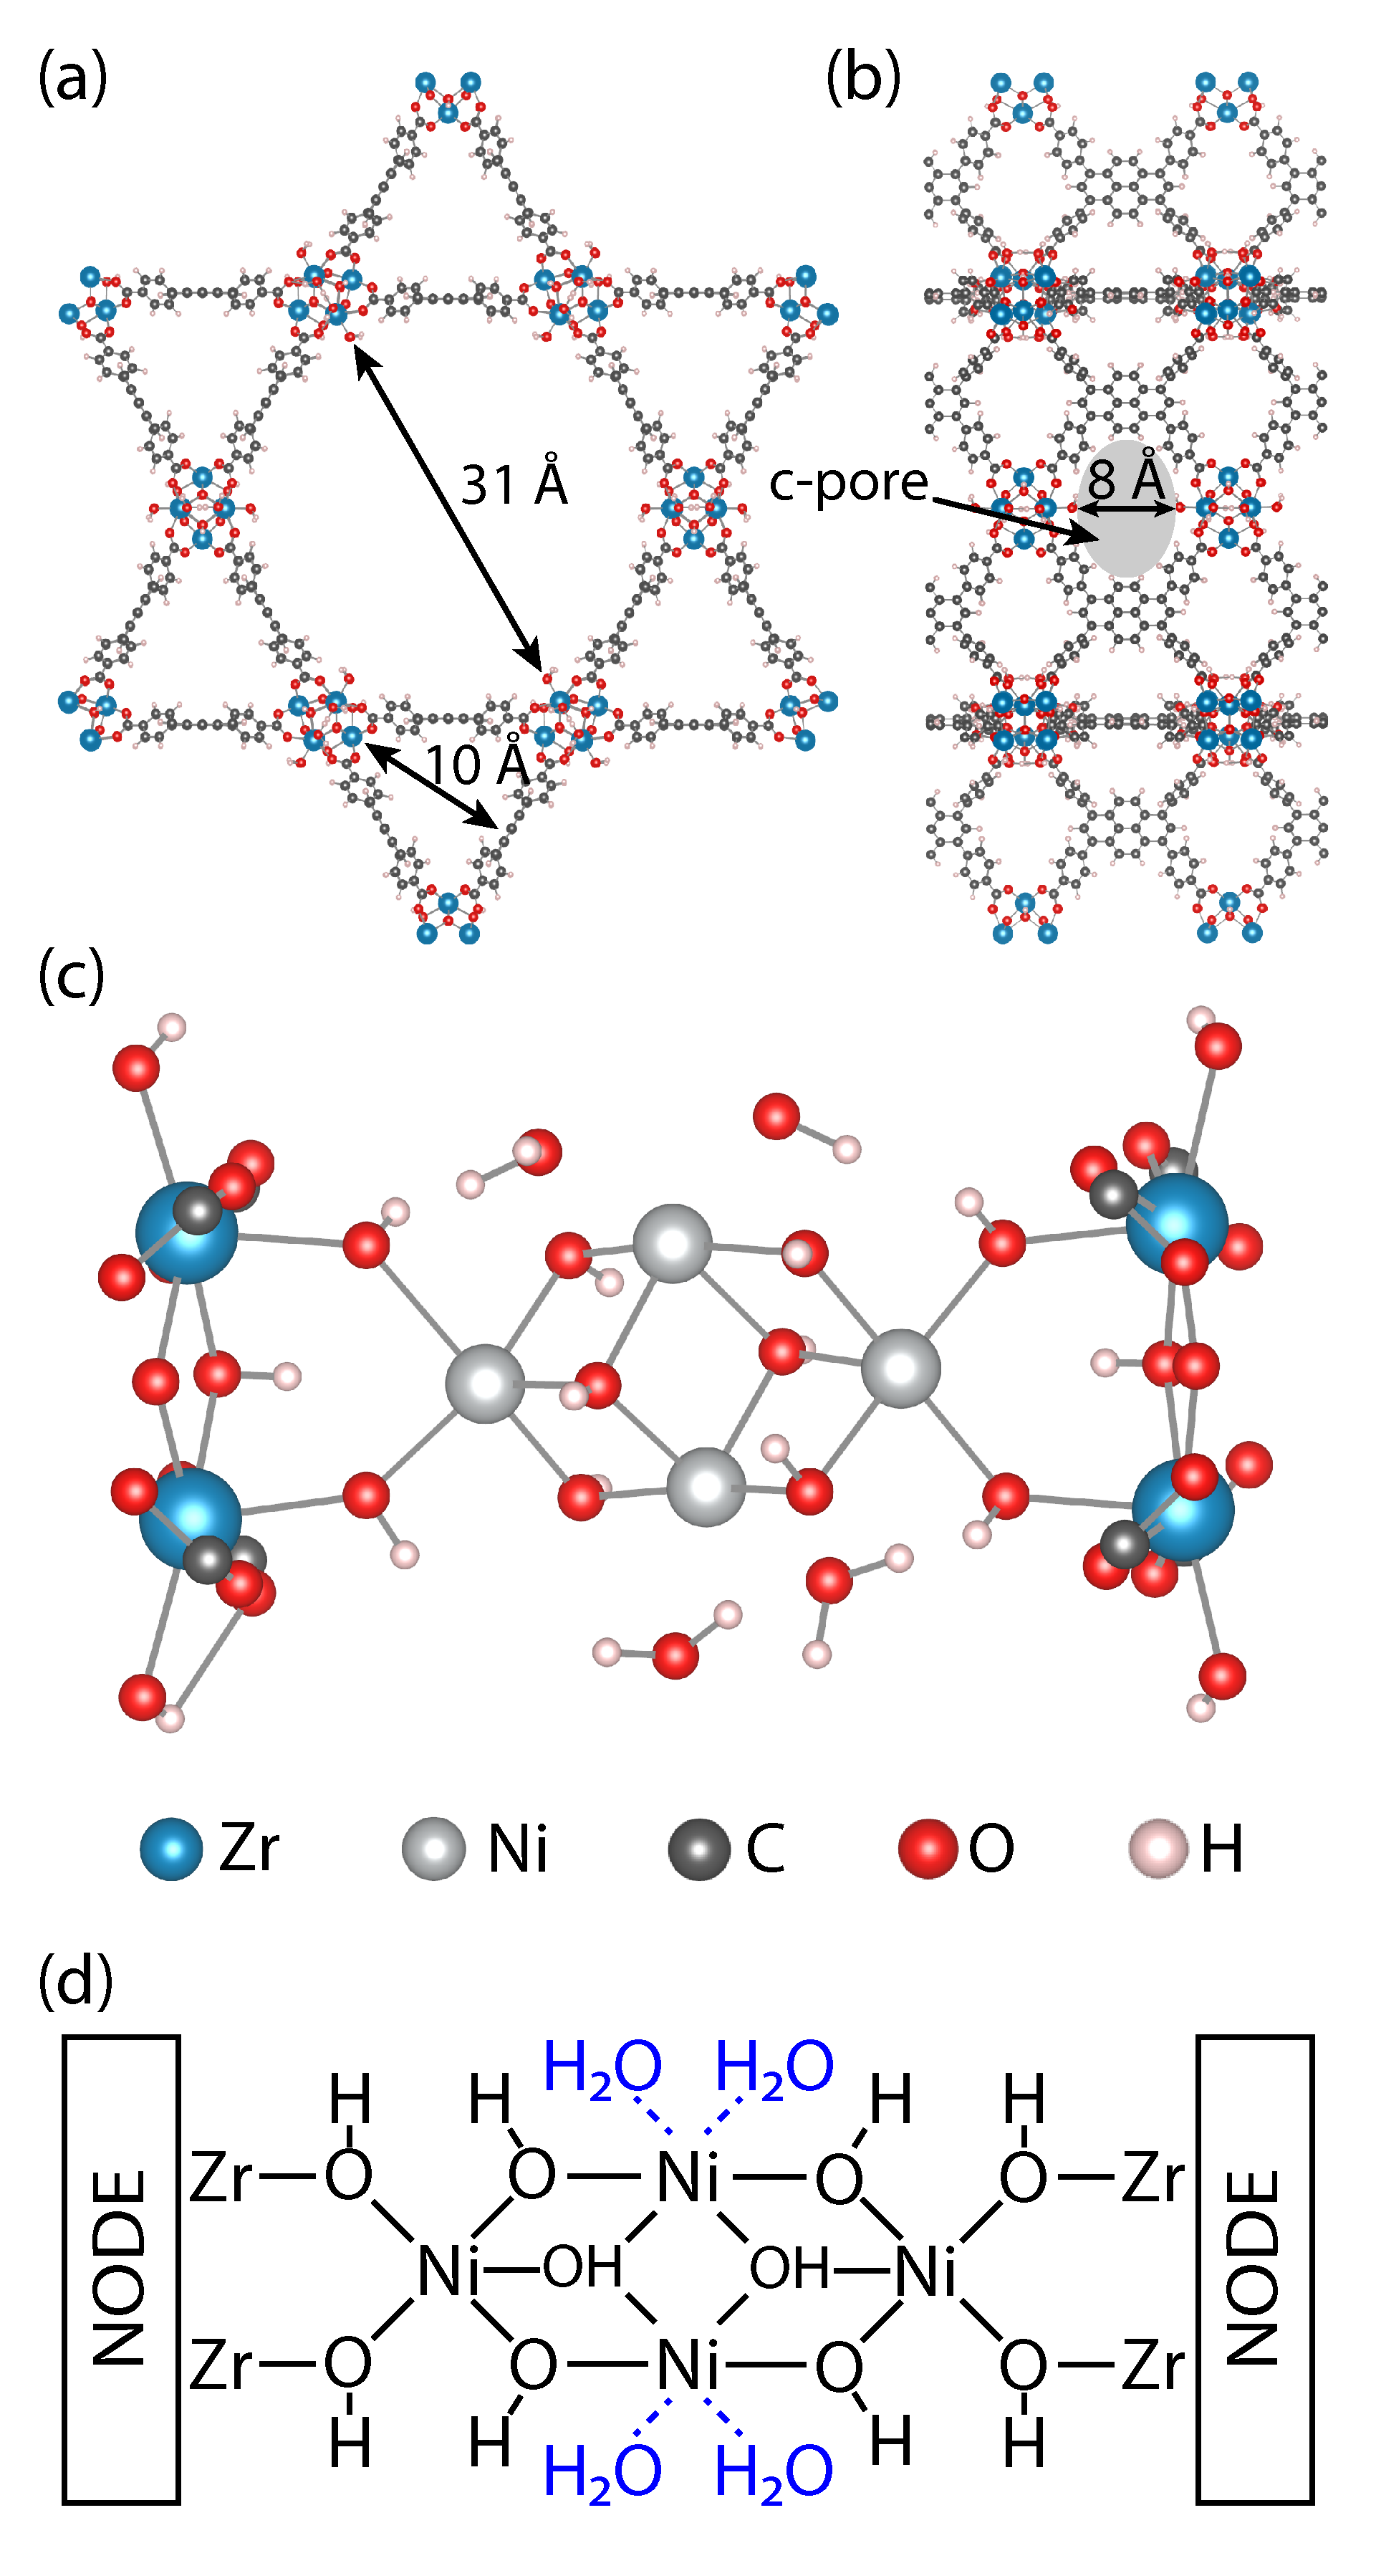
\includegraphics[width=3.0in]{zi-images/00-General-Graphics/2021-figure-MOF-structure.png}
    \caption{
    The structure of NU-1000 shown along the (a) c-axis and the (b) a-axis with the location of the metal complex location highlighted by the gray oval in (b). The gray oval spans the c-pore of NU-1000 (~10 {\AA}). Different variations of the \ce{Ni4}-cluster are shown in (c) and (d) with the node of the MOF framework truncated from the renderings. All adsorbed \ce{H2O} molecules are outlined in blue. 
    }
    \label{fig:Ni-MOF-model}
\end{figure}

\ce{Ni} catalyst models are constructed within the the NU-1000 ``c-pore" (Figure~\ref{fig:Ni-MOF-model}b) following prior work.\cite{PlateroPrats2017} Furthermore, \citeauthor{Ye2017} suggests that the \ce{Ni4}-clusters formed within the ``c-pore" are attached to adjacent nodes.\cite{Ye2017} The two \ce{Ni} ions that bind to the \ce{Zr} nodes each replace one proton (from a \ce{OH/OH2} pair) thereby giving the NU-1000 MOF a net formal charge of $-$2 and the \ce{Ni} catalyst model a net formal charge of $+$2. The \ce{Ni} catalyst models adopt a variety of compositions and comprise between two and four \ce{Ni} ions (denoted as \ce{Ni^{*}} in this work) as well as hydroxyl, water, and hydride ligands. Hydroxyl ligands are denoted \ce{OH^{*}}. Hydride ligands are denoted \ce{H^{*}} and indicate H adsorption onto \ce{Ni^{*}}. Water ligands are denoted \ce{H2O^{*}} and indicate \ce{H} adsorption onto \ce{OH^{*}}. In all, we evaluated \textbf{\color{red}XXX} structures; \textbf{\color{red}the full library can be accessed on our GitHub page.} 

The most thermodynamically stable structures are identified by computing their free energies at different temperatures, partial pressures (of \ce{H2} and \ce{H2O}; see below), and chemical potentials.\cite{Reuter2003,Reuter2004,Grundner2015,Paolucci2016,Li2016,Getman2008,Mandal2020,Zuo2016}
\begin{equation}
    \begin{split}
        \Delta F^{(3)}(\mu_{\text{H}^{*}},\mu_{\text{OH}^{*}},\mu_{\text{Ni}^{*}},V,T)  
        & = \Delta E(N_{\text{H}^{*}},N_{\text{OH}^{*}},N_{\text{Ni}^{*}},V,T) - (\mu_{\text{H}^{*}})(\Delta N_{\text{H}^{*}}) \\ 
        & - (\mu_{\text{OH}^{*}})(\Delta N_{\text{OH}^{*}}) - (\mu_{\text{Ni}^{*}})(\Delta N_{\text{Ni}^{*}}) \\ 
    \end{split}
    \label{eq:free-energy-trans}
\end{equation}
where $F$ is Helmholtz free energy, $E$ is the DFT-calculated electronic energy, $\mu$ is chemical potential, $V$ is volume, $T$ is temperature, and $N$ is number. For example, $N_{\text{H}^*}$ is the number of hydride ligands on the catalyst model. The (3) superscript on $F^{(3)}$ indicates the third Legendre transform, i.e., of $N_{\text{H}^{*}}$, $N_{\text{OH}^{*}}$, and $N_{\text{Ni}^{*}}$ to $\mu_{\text{H}^{*}}$, $\mu_{\text{OH}^{*}}$, and $\mu_{\text{Ni}^{*}}$, respectively. The $\Delta$'s in Eq.~\ref{eq:free-energy-trans} indicate quantities taken relative to a reference structure. The \ce{Ni4(OH)6.4H2O} structure (Figure~\ref{fig:Ni-MOF-model}c and \ref{fig:Ni-MOF-model}d) is used as the reference structure in this work (however, this choice is arbitrary). \ce{H$^*$} and \ce{OH$^*$} are assumed to be in equilibrium with \ce{H2(g)} and \ce{H2O(g)}; hence, chemical potentials of \ce{H$^*$} and \ce{OH$^*$} can be related to chemical potentials of \ce{H2(g)} and \ce{H2O(g)}. Specifically, $\mu_{\text{H}^{*}} = 1/2 \mu_{\text{H}_2(\text{g})}$ and $\mu_{\text{OH}^{*}} = \mu_{\text{H}_2\text{O}(\text{g})} - \mu_{\text{H}^{*}}$. Additionally, the chemical potential of \ce{H2O$^*$} is related to \ce{H2O(g)} using the  $\mu_{\text{H}_2\text{O}(\text{g})} = \mu_{\text{\ce{H2O}}^{*}}$ equilibrium expression. The gas phase chemical potentials are calculated by correcting calculated electronic energies from DFT with free energy contributions from the literature, following prior work.\cite{Reuter2003,Reuter2004,Grundner2015,Paolucci2016,Li2016,Getman2008,Mandal2020} For example,  

\begin{equation}
    \mu_{\text{H}_{2}}^{\text{g}}(T,P_{\text{H}_{2}}) = E_{\text{H}_{2}} + \left[ G_{\text{H}_{2}}(T,P^{o}) - G_{\text{H}_{2}}(0~\text{K},P^{o}) + RT \ln{\left( \frac{P_{\text{H}_{2}}}{P^{o}} \right)} \right]  
    \label{eq:chemicalpotentialrel}
\end{equation}
where $G$ are Gibbs free energies computed using the NASA Polynomials\cite{Mcbride1993} in the pMuTT\cite{LYM2019106864} Python package, $P$ is partial pressure, and $P^{o}$ is the standard pressure (1 bar). Full descriptions of how $E_{\text{H}_2}$ and $E_{\text{H}_2\text{O}}$ are calculated are provided in Supporting Information. In Eq.~\ref{eq:chemicalpotentialrel}, $G(0~\text{K},P^{o})$ is approximated as $G(10~\text{K},P^{o})$, obtained by extrapolating the NASA Polynomials, following prior work.\cite{Getman2008,Li2016}  \ce{Ni$^*$} is assumed to be in equilibrium with bulk Ni, so that $\mu_{\text{Ni}^{*}} = \mu_{\text{Ni}(\text{s})}$. The chemical potential of \ce{Ni(s)} is set equal to $E_\text{Ni(s)}$, following prior work.\cite{Li2016} A full description of how $E_\text{Ni(s)}$ is calculated is provided in Supporting Information. Further details about the thermodynamic modeling approach as well as sensitivity analyses for the various modeling decisions are provided in \hl{supporting information}.

Electronic energies are calculated using the CP2K software package.\cite{Hutter2014} The exchange correlation energy is calculated with the PBE functional\cite{Perdew1996} and corrected using damped D3 dispersion corrections formulated by \citeauthor{Grimme2010}\cite{Grimme2010} The DZVP-MOLOPT basis set is used to model the valance electrons, and the Goedecker pseudopotentials\cite{Goedecker1996} are used to model the core electrons. The plane wave cutoff energy is 360 Ry. The Unrestricted Kohn-Sham (UKS) method is employed given the open shell natures of the \ce{Ni} ions. For example, a single \ce{Ni(II)} ion can adopt either a singlet or triplet state; therefore, clusters with four \ce{Ni} ions can adopt singlet, triplet, quintet, septet, or nonet states. We consider all possible spin states for each catalyst composition, given the importance of the spin state on the computed electronic energy.\cite{Shabbir2020,Ye2017,Bernales2016,Mandal2020} Any spin state exhibiting spin contamination is removed from thermodynamic analysis (see supporting information for more details). The final of $E$ used in thermodynamic analysis are obtained from geometry relaxations where all atoms in the periodic unit cell are allowed to relax. A sample input file for the CP2K calculations is provided in Supporting Information.

The pair distribution function (PDF), G(r), represents the local structure as a histogram atom-atom distances in the material weighted by the scattering power of the atoms involved. While the measured PDF reflects all atom-atom distances within the material, by deriving a differential PDF (dPDF), where the PDF measured for NU-1000 is subtracted from the PDF measured for the Ni-complex containing Ni-NU-1000, we analytically isolate the atom-atom distances that define the \ce{Ni} cluster and its interaction with NU-1000 support. Thus the dPDF includes the interatomic distances  within the cluster (\ce{Ni{\Compactcdots}Ni}, \ce{Ni-O}, \ce{O{\Compactcdots}O} atom pairs) and between the cluster and the MOF (\ce{Ni{\Compactcdots}Zr} and \ce{Ni{\Compactcdots}O}) with atom pairs not directly bonded to each other receiving the ``${\Compactcdots}$" notation. PDFs of the computed structural models were simulated within PDFgui using typical values of instrument and atomic displacement parameters for such materials. Given the lower scattering contribution from the \ce{O} atoms compared to \ce{Ni} atoms, \ce{O{\Compactcdots}O} pairs have very low contribution to the measured data and were not calculated. The simulated PDFs were evaluated for their correspondence to the experimental data over XYZ {\AA} range. The experimental details of the PDF measurements are described elsewhere in detail.\cite{PlateroPrats2017} The tetranuclear \ce{Ni} cluster exposed to \ce{H2} (3.5\% in \ce{He}) at 200 \degree C for 2 hours and then cooled to 50 \degree C in \ce{H2} for measurement.\cite{PlateroPrats2017} Powder X-ray diffraction (XRD) and total scattering data suitable for PDF analysis were collected at 50 \degree C in \ce{H2}.

%%%%%%%%%%%%%%%%%%%%%%%%%%%%%%%%%%%%%%%%%%%%%%%%%%%%%%%%%%%%%%%%%%%%%
%% Results
%%%%%%%%%%%%%%%%%%%%%%%%%%%%%%%%%%%%%%%%%%%%%%%%%%%%%%%%%%%%%%%%%%%%%
\section{Results}
The dPDF for the experimentally obtained structure is shown in Figure~\ref{fig:dPDFs_TandP_trans_Ni}. The dPDFs provide structural insights into the cluster by revealing key interatomic distances with peaks indicating the distance between different atoms. First coordination sphere distances are reported using a line (e.g., \ce{Ni-O}) while second coordination sphere distances are reported using dots (e.g., \ce{Ni{\Compactcdots}Ni} and \ce{Ni{\Compactcdots}Zr}. The significant peaks in the experimental structure are the \ce{Ni-O} distance at 2.02 {\AA}, the \ce{Ni{\Compactcdots}Ni} distances at 3.01 {\AA} and 3.27 {\AA}, and the \ce{Ni{\Compactcdots}Zr} distances at 3.78 {\AA} and 4.08 {\AA}, yielding a Ni coordination number of ca. 5. The ``double" peaks at 3.01 {\AA} and 3.27 {\AA} and 3.78 {\AA} and 4.08 {\AA} indicate asymmetric interatomic distances with the cluster, suggesting that structurally similar Ni ions coordinate to different ligands. For example, our models comprising four Ni ions contain two types of Ni ions: two that connect to the Zr nodes and two that do not (e.g., see Figures~\ref{fig:Ni-MOF-model}(c), \ref{fig:Ni-MOF-model}(d), and \ref{fig:Ni-structure-diagram}). To exhibit asymmetry, we expect (i) the two Ni ions that connect to the Zr nodes will have coordination environments that differ from each other, and (ii) the two Ni ions that do not connect to the Zr nodes will have coordination environments that differ from each other. 

% Structure Diagram
\begin{figure}[H]
    \centering
    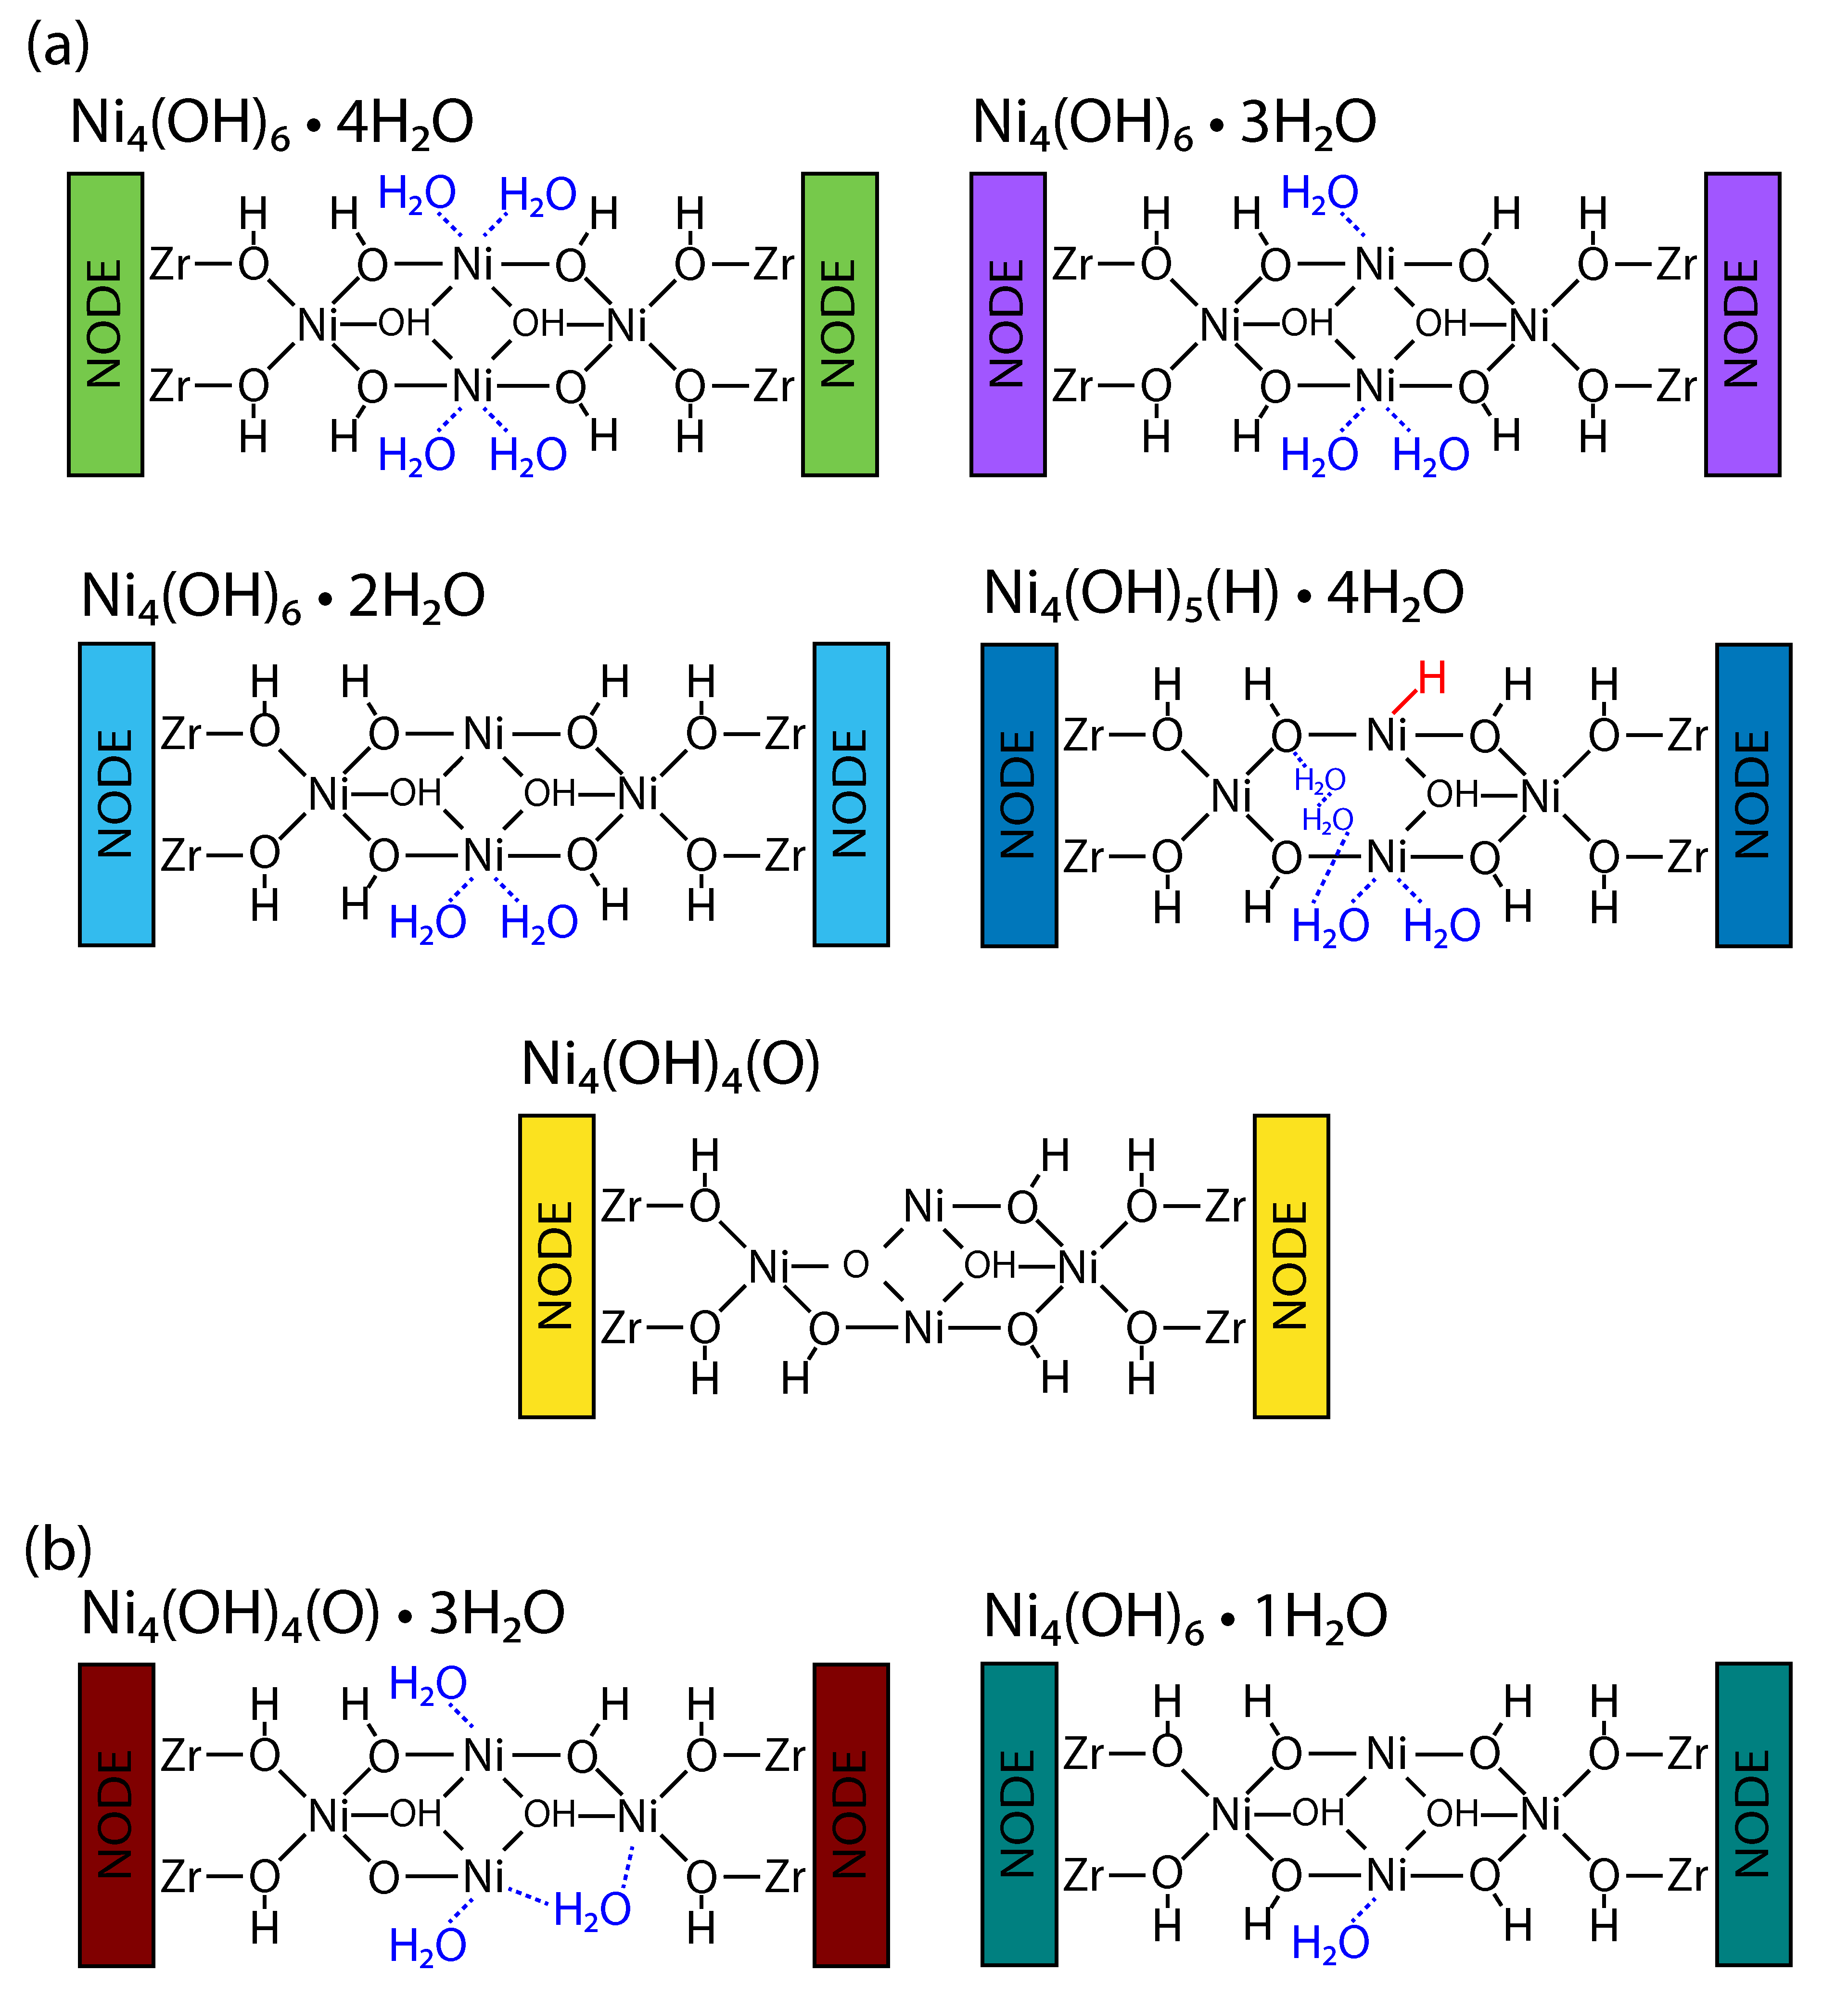
\includegraphics{zi-images/01-Ni-Graphics/2021-MAIN-structure-diagram.png}
    \caption{
    Depictions of key structures considered in this work along with the names used to identify them. The color and numbering schemes are the same as in Figures~\ref{fig:dPDFs_TandP_trans_Ni} and \ref{fig:phase_diagram_Ni_combined}. Structure denoted with an $\blacklozenge$ are not thermodynamic minimum under any of the explored conditions.
    }
    \label{fig:Ni-structure-diagram}
\end{figure}

% dPDF diagram for the phase diagram structures 
\begin{figure}[H]
    \centering
    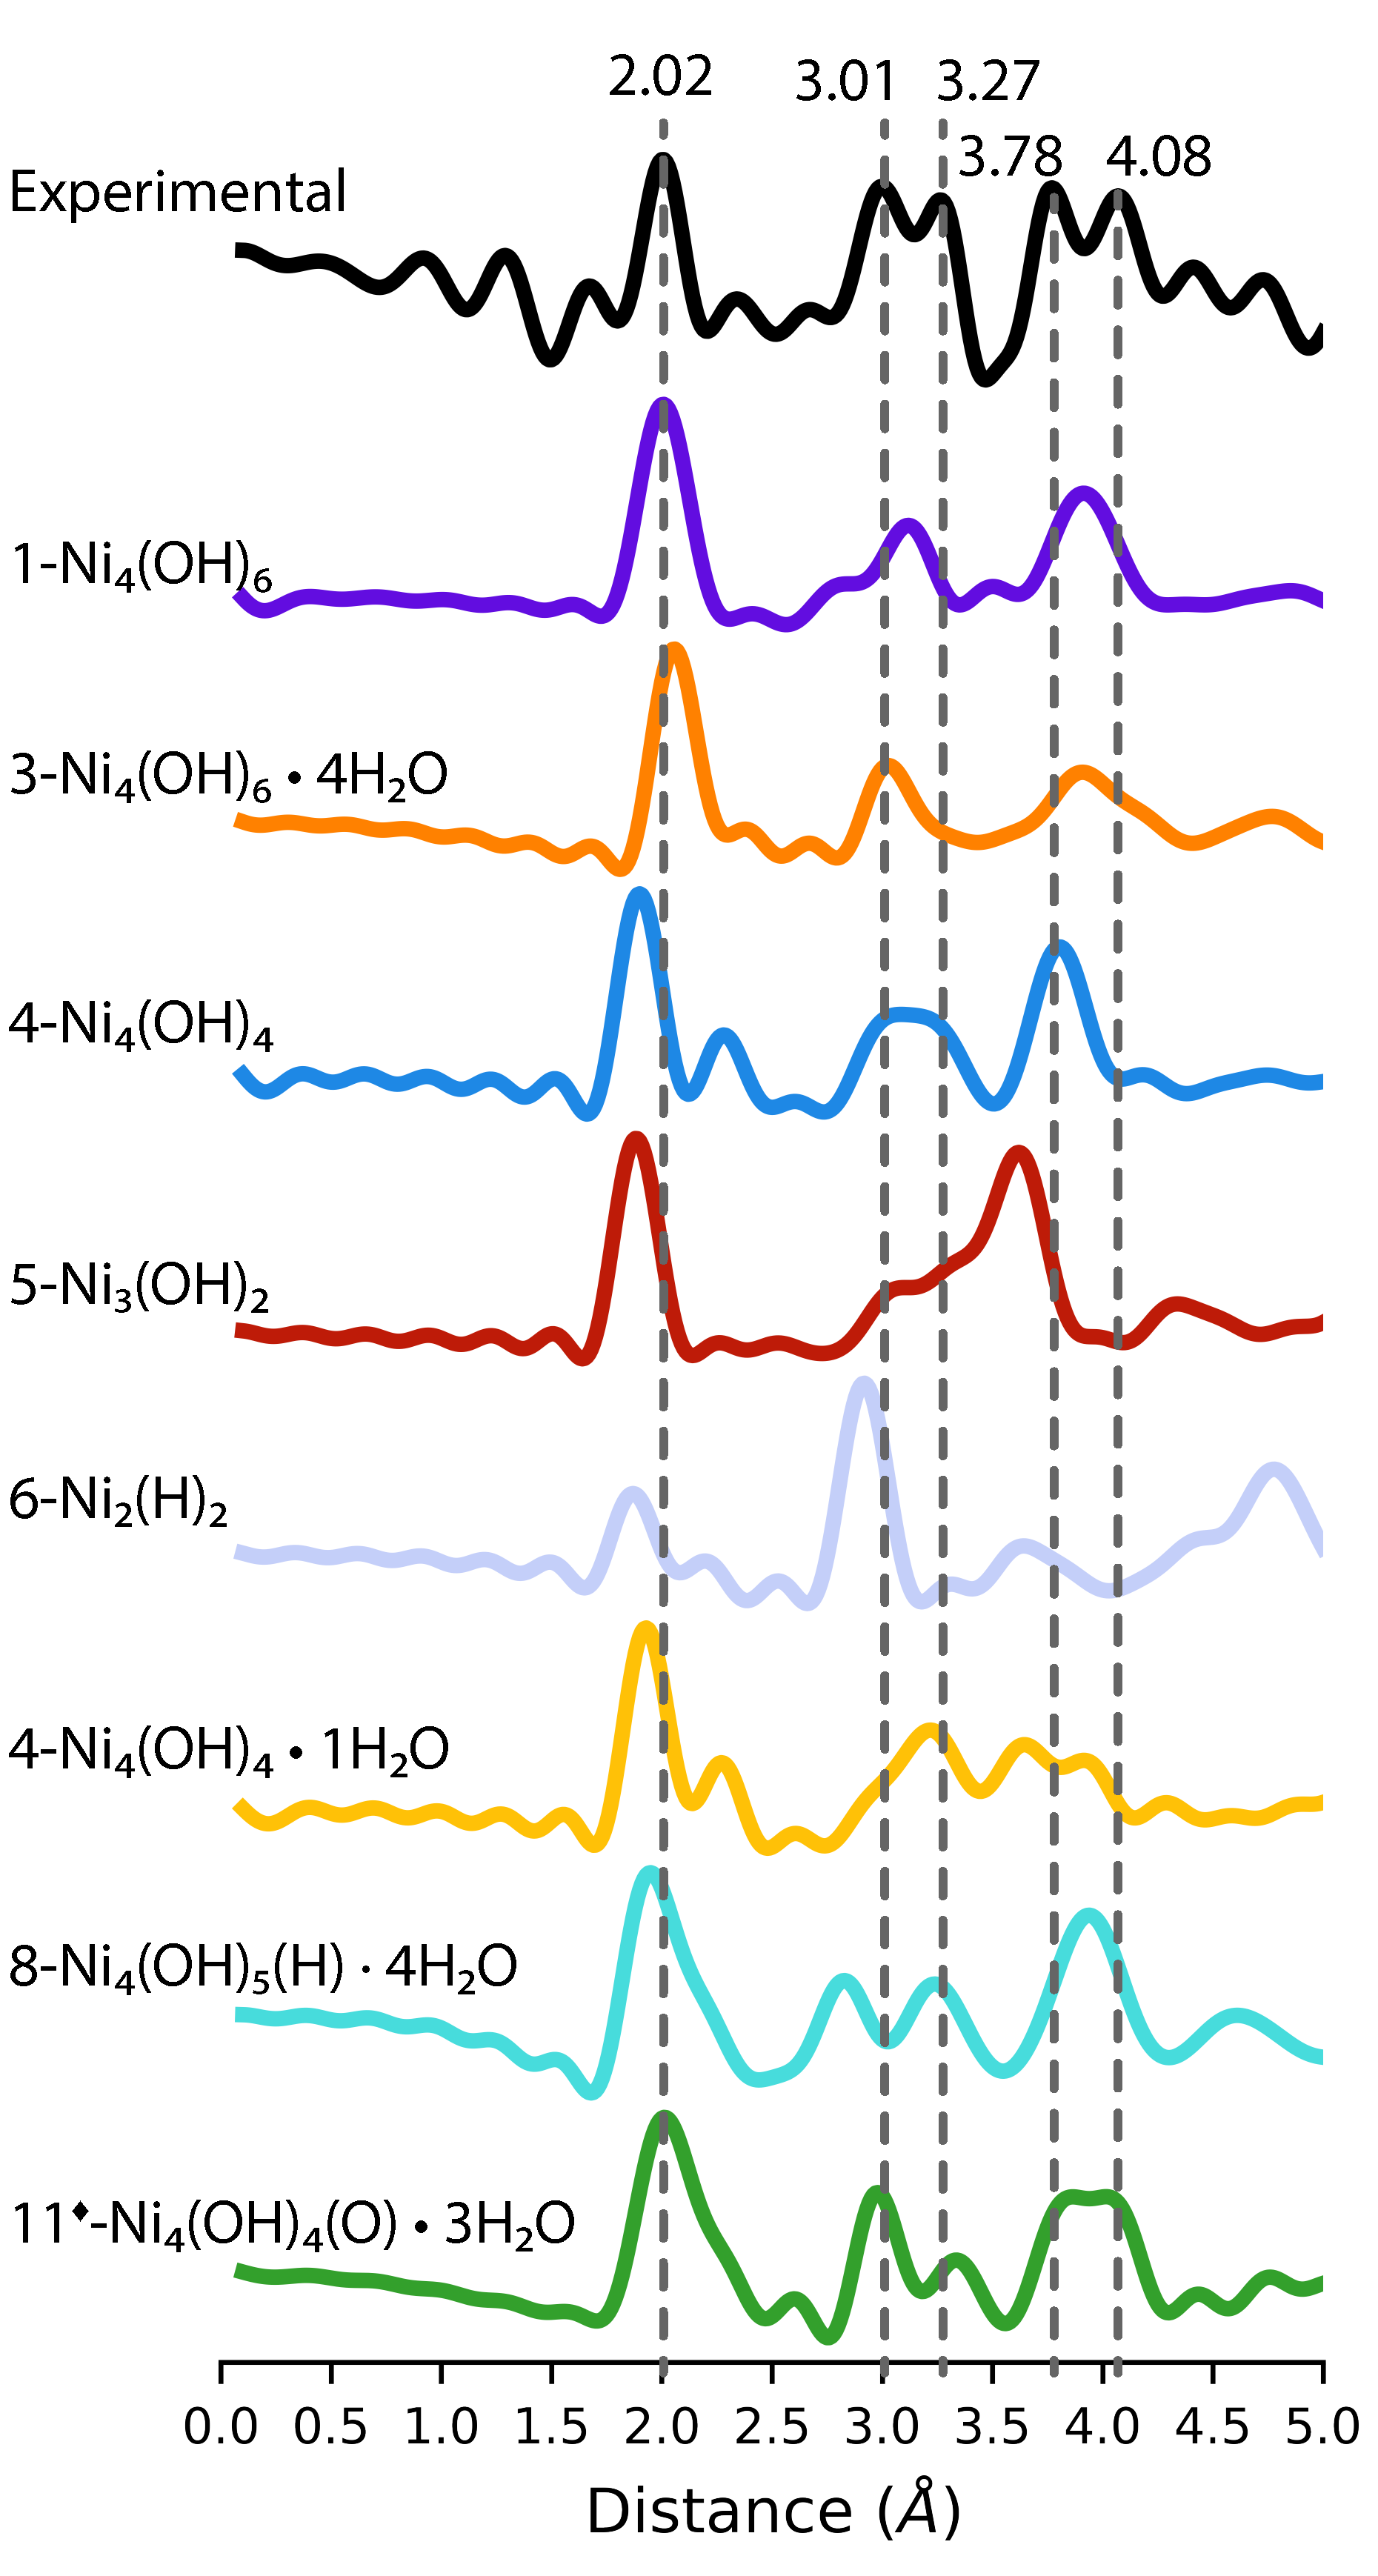
\includegraphics{zi-images/01-Ni-Graphics/2021-MAIN-single-dPDF-highH2O.png}
    \caption{
    Differential pair distribution functions (dPDFs) for experimental and simulated structures considered in this study. The color and numbering schemes are the same as in Figures~\ref{fig:Ni-structure-diagram} and \ref{fig:phase_diagram_Ni_combined}.  
    }
    \label{fig:dPDFs_TandP_trans_Ni}
\end{figure}

Thermodynamic analysis is used to provide atomic-level insight into the Ni cluster composition and structure. Based on the observation from experiments that the Ni ions are highly coordinated, we perform thermodynamic analysis at significant $P_{\text{\ce{H2O}}}$ of $10^{-1}$ bar. This choice is justified below; further, sensitivity of the results to this choice is provided in Supporting Information. Phase diagrams for the Ni cluster calculated as a function of $T$ and $P_{\text{\ce{H2}}}$ are provided in Figure~\ref{fig:phase_diagram_Ni_combined} (with corresponding structures depicted in Figure~\ref{fig:Ni-structure-diagram}). In general, increasing \ce{H2} partial pressure results in conversion of $\ce{OH^{*}}$ to $\ce{H2O^{*}}$ and in some cases formation of $\ce{H^{*}}$. It also promotes loss of $\ce{Ni^{*}}$ (see Figure~\ref{fig:phase_diagram_Ni_combined}(a)).  

% The combined phase diagram figures
\begin{figure}[H]
    \centering
    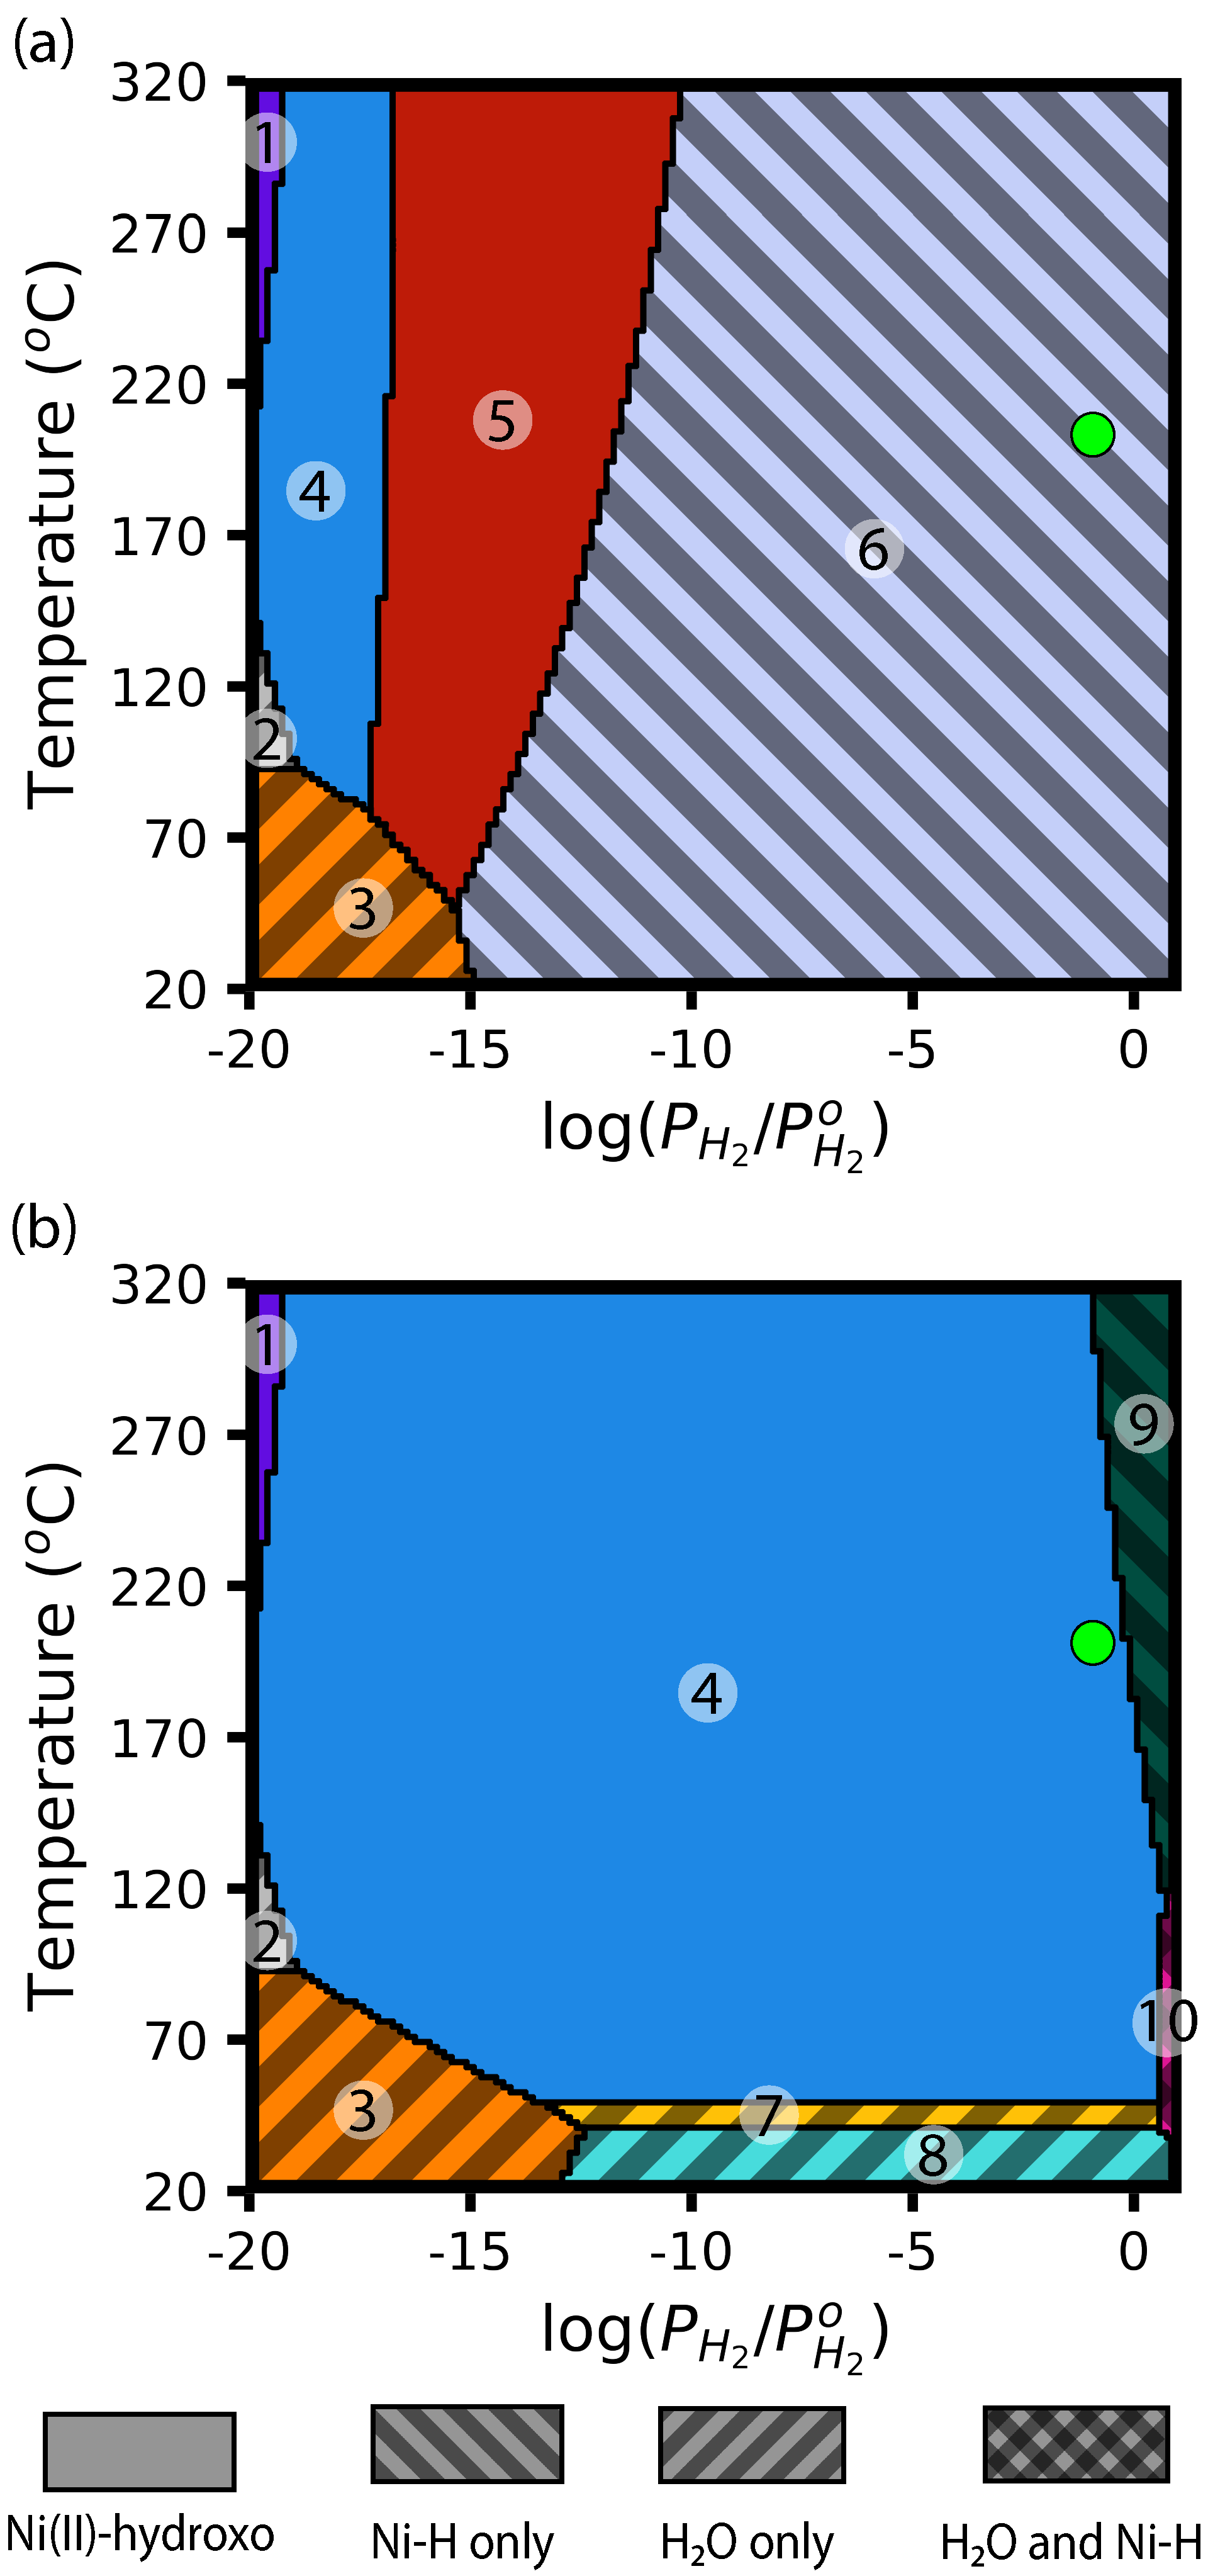
\includegraphics{zi-images/01-Ni-Graphics/2021-MAIN-phase-diagram-combined.png}
    \caption{
    Phase diagrams for the Ni cluster catalyst calculated at $P_{\text{\ce{H2O}}}=10^{-1}$ bar as a function of $T$ and $P_{\text{H}_2}$. (a) Variable Ni composition. (b) Ni composition fixed at 4 Ni ions. The different structures are represented by the different colored and numbered regions; the color and numbering schemes are the same as in Figures~\ref{fig:dPDFs_TandP_trans_Ni} and \ref{fig:Ni-structure-diagram}. In (a), $\mu_{\text{Ni(s)}}$ is fixed (= $E_{\text{Ni(s)}}$), whereas in (b), $N_{\text{Ni(s)}}$ is fixed (= 4).
    }
    \label{fig:phase_diagram_Ni_combined}
\end{figure}   

Of interest is the catalyst composition and structure under operating conditions, i.e., 0.1~bar \ce{H2} and $T \le$~200~K. The structure that minimizes $F^{(3)}$ at these conditions, according to Figure~\ref{fig:phase_diagram_Ni_combined}(a), i.e., where the compositions of hydride, hydroxyl, and water ligands as well as Ni ions are allowed to vary, is 6-\ce{Ni2(H)2} (lilac in Figure~\ref{fig:Ni-structure-diagram}). This structure features two isolated single Ni ion hydride structures, similar to models used in prior catalytic studies.\cite{Li2016sintering,Shabbir2020, Hackler2020} However, the dPDF for this structure is in stark contrast with the experimental dPDF, given its low Ni coordination number of ca. 3. Further, the dPDF for the lilac structure does not match well with the experimentally observed one. In fact, given that removal of Ni only occurs after significant depletion of $\ce{OH^{*}}$, which in turn decreases the Ni coordination number, the only structures from our library that have the possibility of matching the experimental dPDF are those with four Ni ions. Hence, Figure~\ref{fig:phase_diagram_Ni_combined}(b) provides a phase diagram where the number of Ni ions is held fixed at 4. 

While several structures on this phase diagram exhibit \ce{Ni-O} peaks in good agreement with experiment, only one, 8-\ce{Ni4(OH)5(H).4H2O} (teal in Figure~\ref{fig:Ni-structure-diagram}), exhibits double \ce{Ni{\Compactcdots}Ni} peaks. This ``teal" structure features hydride, hydroxyl, and water ligands as well as \ce{H2O} molecules that form a hydrogen bonded chain between a hydroxyl ligand and a water ligand and is the thermodynamically preferred structure under conditions of relevance to catalysis. We determined the binding energy of the \ce{H2O} molecule that is uncoordinated to any cluster \ce{Ni} atoms in the chain is -104 kJ/mol, which is lower in energy than \ce{H2O} coordinated to \ce{Ni} (~-75 kJ/mol). The more favorable binding energy suggests that despite not being coordinated to any \ce{Ni}, that the \ce{H2O} has favorable interactions with other parts of the MOF. The distance between a carbon atom in pyrene-linker and the \ce{H} atom in the \ce{H2O} molecules is 2.37 {\AA} and 2.70 {\AA}, respectively.   

While this structure captures double peaks for the \ce{Ni{\Compactcdots}Ni} distances, it is still not a good match with experiment, as it underpredicts the \ce{Ni-O} distance, features a shifted \ce{Ni{\Compactcdots}Ni} peak splitting, and contains a single \ce{Ni{\Compactcdots}Zr} peak. We hence searched our structural database for structures that more closely matched the \ce{Ni{\Compactcdots}Ni} peak splitting. The structure from our library that gave the best agreement with the experimental dPDFs is 14*-\ce{Ni4(OH)4(O).3H2O} (green). It should be noted that this structure is not a thermodynamic minimum, according to our analysis, which is why it does not appear on the phase diagram. This ``green" structure comprises hydride, hydroxyl, and water ligands and additionally includes a \ce{\mu_{2}-O} ligand instead of a \ce{\mu_{2}-OH} ligand. Although not as pronounced, the green structure demonstrates both \ce{Ni{\Compactcdots}Ni} and \ce{Ni{\Compactcdots}Zr} peak splitting. While this structure still does not reproduce the experimental dPDF, it provides clues as to the composition and structure of the Ni cluster under catalytic operating conditions. 

%%%%%%%%%%%%%%%%%%%%%%%%%%%%%%%%%%%%%%%%%%%%%%%%%%%%%%%%%%%%%%%%%%%%%
%% Discussion
%%%%%%%%%%%%%%%%%%%%%%%%%%%%%%%%%%%%%%%%%%%%%%%%%%%%%%%%%%%%%%%%%%%%
\subsection{Discussion}
Taking together the experimental and computational results, several things about the Ni cluster structure become clear. First, Ni is highly coordinated, as evidenced by the experimental dPDF. Our thermodynamic modeling indicates that for this condition to be met, catalysts must comprise a significant Ni content, since removal of Ni is caused by removal of $\ce{OH^{*}}$ ligands (and hence reduction in the Ni coordination number). Presence of $\ce{OH^{*}}$ ligands is also important, since they hold the structure together. In our model, this indicates appreciable $\mu_{\text{H}_2\text{O}(\text{g})}$.  $\ce{H2O^{*}}$ ligands seem to also play a role in causing \ce{Ni{\Compactcdots}Ni}, and possibly \ce{Ni{\Compactcdots}Zr} peak splitting (\ce{Ni{\Compactcdots}Zr} could also be caused by XXX, which we have not studied in this paper); the two structures (teal and green) that demonstrate peak splitting have 3 (green) and 4 (teal) $\ce{H2O^{*}}$ ligands, respectively. Interestingly, in both of these structures, the $\ce{H2O^{*}}$ ligands bridge two ligands (teal) or Ni ions (green), suggesting that bridging $\ce{H2O^{*}}$ ligands could cause the peak splitting observed experimentally. 


Interestingly, few of the structures on Figure \ref{fig:phase_diagram_Ni_combined} comprise hydride ligands, which have been previously suggested as the active site in hydrogenation catalysis. While this work does not rule out metal hydrides as active sites, it suggests that other ligands, e.g., \ce{OH} or \ce{H2O} ligands, could participate in the active site for catalysis.  The lack of \ce{Ni-H} raises questions about the catalytically active group for the \ce{Ni} metal complex catalyst. 


\subsection{Conclusions}
We present the rich structural landscape of a \ce{Ni} metal complex using a \textit{ab initio} thermodynamic analysis, which combines density functional theory (DFT) and empirical gas phase thermochemistry to determine the thermodynamic stability of a \ce{Ni} metal complex at different conditions. We explore the influence of temperature, \ce{H2O} partial pressure, and \ce{H2} partial pressure on the thermodynamic stability and report our finding as phase diagrams. We quantify the local structures of our model using dPDF analysis, and compare our model structures to experimental dPDF for a \ce{Ni} metal complex supported on NU-1000. Comparisons with experiments reveal the importance of a high \ce{Ni} coordination environment, which is maintained by coordinated \ce{OH} and \ce{H2O} groups to the \ce{Ni} atoms of the cluster. When exposed to \ce{H2} and elevated temperatures, our model shows the removal of \ce{OH} ligands, resulting in lower \ce{Ni} coordination within the active site. Structures with a low \ce{Ni} coordination generate peaks that are not observed experimentally. With a higher \ce{H2O} partial pressure, our \textit{ab initio} thermodynamic modeling produce structures that include both \ce{OH} and \ce{H2O} species within the active site. We expand from structures that are thermodynamic minima to include other structures within the library. A general trend is that the structures containing more \ce{OH} and \ce{H2O} groups show better agreement to the experimental dPDF in our dPDF analysis, and these structures become thermodynamically relevant at higher \ce{H2O} partial pressures. 

 Overall, the findings establish improve models that require further computational catalytic investigations, including the exploration of the kinetic barriers related to these transformations.
 
\subsection{References}

%The class makes various changes to the way that references are
%handled.  The class loads \textsf{natbib}, and also the
%appropriate bibliography style.  References can be made using
%the normal method; the citation should be placed before any
%punctuation, as the class will move it if using a superscript
%citation style
%\cite{Mena2000,Abernethy2003,Friedman-Hill2003,EuropeanCommission2008}.
%The use of \textsf{natbib} allows the use of the various citation
%commands of that package: \citeauthor{Abernethy2003} have shown
%something, in \citeyear{Cotton1999}, or as given by
%Ref.~\citenum{Mena2000}.  Long lists of authors will be
%automatically truncated in most article formats, but not in
%supplementary information or reviews \cite{Pople2003}. If you
%encounter problems with the citation macros, please check that
%your copy of \textsf{natbib} is up to date. The demonstration
%database file \texttt{achemso-demo.bib} shows how to complete
%entries correctly. Notice that ``\latin{et al.}'' is auto-formatted
%using the \texttt{\textbackslash latin} command.

%Multiple citations to be combined into a list can be %given as
%a single citation.  This uses the \textsf{mciteplus} %package
%\cite{Johnson1972,*Arduengo1992,*Eisenstein2005,*Arduengo%1994}.
%Citations other than the first of the list should be %indicated
%with a star. If the \textsf{mciteplus} package is not %installed,
%the standard bibliography tools will still work but %starred
%references will be ignored. Individual references can be %referred
%to using \texttt{\textbackslash mciteSubRef}:
%``ref.~\mciteSubRef{Eisenstein2005}''.

%The class also handles notes to be added to the bibliography.  These
%should be given in place in the document \bibnote{This is a note.
%The text will be moved the the references section.  The title of the
%section will change to ``Notes and References''.}.  As with
%citations, the text should be placed before punctuation.  A note is
%also generated if a citation has an optional note.  This assumes that
%the whole work has already been cited: odd numbering will result if
%this is not the case \cite[p.~1]{Cotton1999}.

%%%%%%%%%%%%%%%%%%%%%%%%%%%%%%%%%%%%%%%%%%%%%%%%%%%%%%%%%%%%%%%%%%%%%
%% The "Acknowledgement" section can be given in all manuscript
%% classes.  This should be given within the "acknowledgement"
%% environment, which will make the correct section or running title.
%%%%%%%%%%%%%%%%%%%%%%%%%%%%%%%%%%%%%%%%%%%%%%%%%%%%%%%%%%%%%%%%%%%%%
%\begin{acknowledgement}
%
%\hl{authors would like to thank \ldots''.
%
%The author thanks Mats Dahlgren for version one of \textsf{achemso},
%and Donald Arseneau for the code taken from \textsf{cite} to move
%citations after punctuation. Many users have provided feedback on the
%class, which is reflected in all of the different demonstrations
%shown in this document.}
%
%\end{acknowledgement}

%%%%%%%%%%%%%%%%%%%%%%%%%%%%%%%%%%%%%%%%%%%%%%%%%%%%%%%%%%%%%%%%%%%%%
%% The same is true for Supporting Information, which should use the
%% suppinfo environment.
%%%%%%%%%%%%%%%%%%%%%%%%%%%%%%%%%%%%%%%%%%%%%%%%%%%%%%%%%%%%%%%%%%%%%
%\begin{suppinfo}
%
%\hl{This will usually read something like: ``Experimental procedures and
%characterization data for all new compounds. The class will
%automatically add a sentence pointing to the information on-line:}
%
%\end{suppinfo}

%%%%%%%%%%%%%%%%%%%%%%%%%%%%%%%%%%%%%%%%%%%%%%%%%%%%%%%%%%%%%%%%%%%%%
%% The appropriate \bibliography command should be placed here.
%% Notice that the class file automatically sets \bibliographystyle
%% and also names the section correctly.
%%%%%%%%%%%%%%%%%%%%%%%%%%%%%%%%%%%%%%%%%%%%%%%%%%%%%%%%%%%%%%%%%%%%%
\bibliography{achemso-demo}

\end{document}